% Generated by run_literature_pi_comparison.m.
\subsubsection{Comparison with a passivity-based PI controller}
We also implement the decentralized multivariable PI voltage controller of Nahata et al.~\cite{Nahata2020}, using its explicit gain region. With $e_{Vi}=V_i-V_{Ei}$ and $e_{Ii}=I_{ti}-I_{tEi}$, its equilibrium-centered realization is
\begin{align}\dot z_i&=-e_{Vi},\nonumber\\ V_{ti}&=V_{Sti}+k_{1i}e_{Vi}+k_{2i}e_{Ii}+k_{3i}z_i,\label{Eq:LiteraturePI}\end{align}
where $k_{1i}<1$, $k_{2i}<R_i$, and $0<k_{3i}<(1-k_{1i})(R_i-k_{2i})/L_i$. The baseline uses the same equilibrium, physical plant, initial errors, and disturbances. Its integral deviations start at zero. We verify the published local storage and the coupled resistive-network dissipation inequality, as well as the complete closed-loop poles.
A saved 125-candidate grid selects $k_{1i}=-2$, $k_{2i}=-0.5$, and $k_{3i}=0.25(1-k_{1i})(R_i-k_{2i})/L_i$. Selection minimizes nominal settling time under a 4.089 V peak command-deviation budget, equal to the larger nominal peak of the two co-designs; the disturbance tests are not used for tuning.
\begin{table}[t]\centering\small\caption{Literature comparison: nominal settling time (ms), and disturbance RMS voltage (V), sharing (p.u.), and command deviation (V).}\label{Tab:LiteraturePI}\begin{tabular}{lrrrr}\hline Method & Settling & Voltage & Sharing & Command\\\hline
MB co-design & 3.30 & 0.1600 & 0.00339 & 0.2611 \\
DD co-design & 3.20 & 0.1520 & 0.00336 & 0.2537 \\
Passivity PI & 7.40 & 0.0484 & 0.00820 & 0.1463 \\
\hline\end{tabular}\end{table}
Figure~\ref{Fig:LiteraturePI} and Table~\ref{Tab:LiteraturePI} compare transient regulation and control effort. A separate persistent-load test adds 0.35 A at every bus at 25 ms while keeping the voltage references fixed. This is a regulation diagnostic, not an $L_2$-gain test.
Over 100--120 ms, the voltage RMS errors are 1.14 V (MB), 1.09 V (DD), and $6.8\times10^{-6}$ V (PI); the corresponding sharing RMS errors are 0.02445, 0.02458, and 0.01994 p.u. The PI integral action enforces zero asymptotic voltage offset, but does not enforce proportional sharing after the load changes. Thus the comparison distinguishes voltage restoration from current-sharing performance. All three controllers use zero communication links here. The PI stability certificate does not provide the synthesized global $L_2$ gain reported for the co-designs.
\begin{figure*}[t]\centering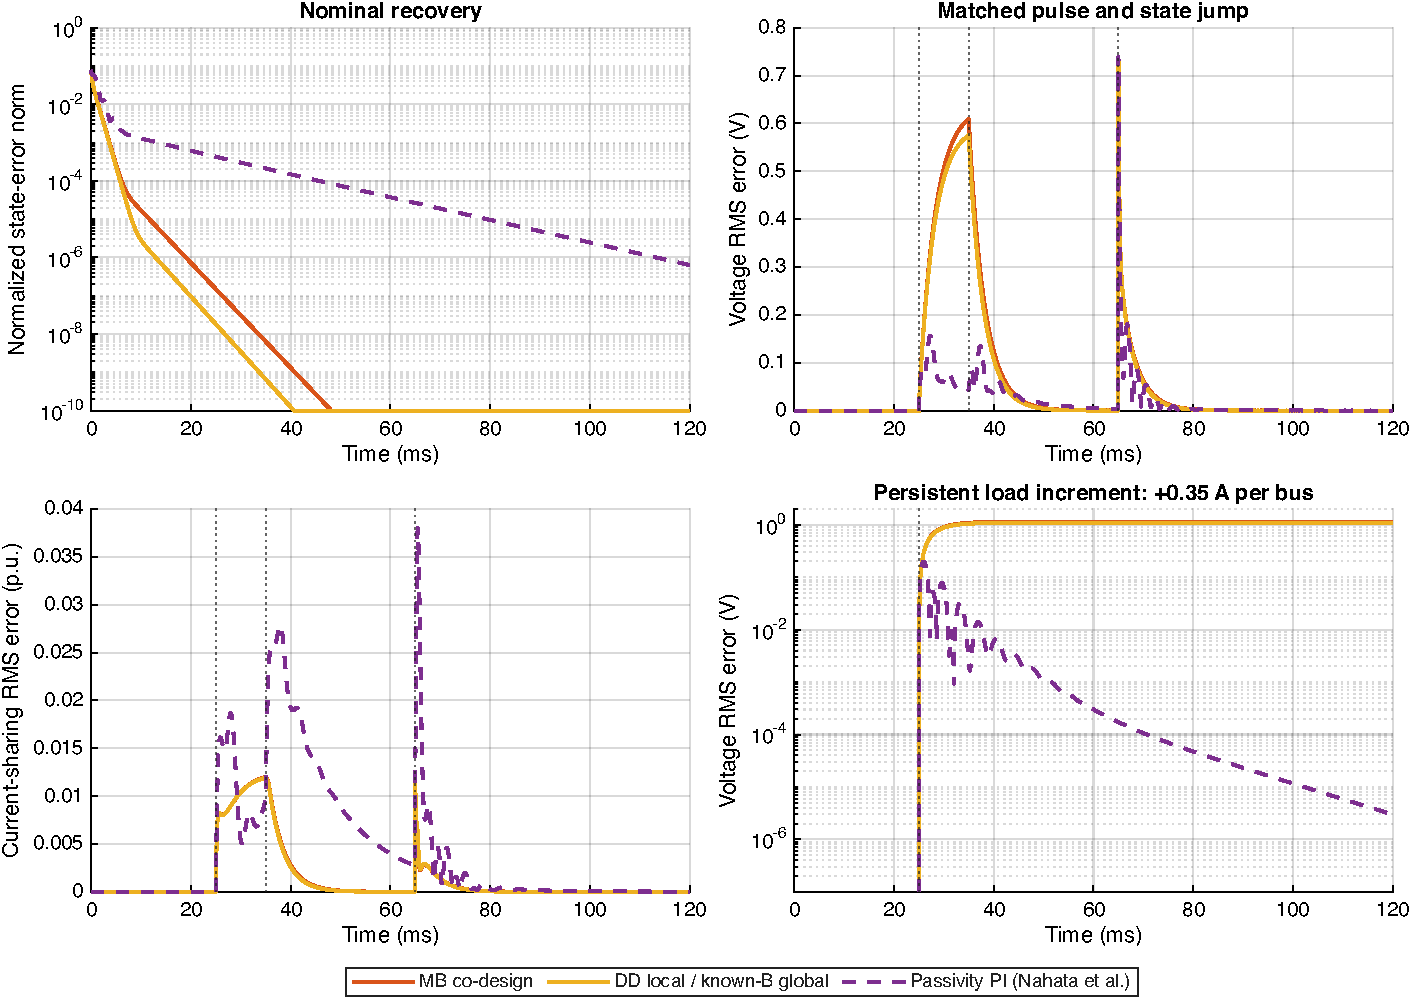
\includegraphics[width=0.86\textwidth]{Results/LiteraturePI/literature_pi_comparison.pdf}\caption{Comparison with the literature PI baseline on the same continuously coupled ZI microgrid. The additional permanent-load experiment exposes the effect of integral voltage restoration.}\label{Fig:LiteraturePI}\end{figure*}
